\documentclass{article}
\usepackage{mathtools}
\usepackage{amsfonts}
\usepackage{amssymb}
\usepackage{fullpage}
\usepackage{amsmath}
\usepackage{multirow}
\usepackage{graphicx}
\usepackage{caption}
\usepackage{subcaption}
\usepackage{float}
\usepackage{hyperref}
\usepackage[utf8]{inputenc}
\usepackage{tikz}
\usetikzlibrary{shapes.geometric, arrows}

\tikzstyle{startstop} = [rectangle, rounded corners, minimum width=3cm, minimum height=1cm,text centered, draw=black, fill=red!30]
\tikzstyle{randomAlaska} = [trapezium, trapezium left angle=80, trapezium right angle=100, minimum width = 1cm, minimum height=1cm, text centered, draw=black, text width = 3cm, node distance=3cm, fill=blue!30]
\tikzstyle{randomArabia} = [trapezium, trapezium left angle=80, trapezium right angle=100, minimum width = 1cm, minimum height=1cm, text centered, draw=black, text width = 3cm, node distance=3cm, fill=red!80]
\tikzstyle{randomCaribbean} = [trapezium, trapezium left angle=80, trapezium right angle=100, minimum width = 1cm, minimum height=1cm, text centered, draw=black, text width = 3cm, node distance=3cm, fill=black!20]
\tikzstyle{process} = [rectangle, minimum width=3cm, minimum height=1cm, text centered, text width=3cm, draw=black, fill=orange]
\tikzstyle{fixedEffects} = [diamond, minimum width=3cm, minimum height=1cm, text centered, draw=black, node distance=3cm, fill=green!30]
\tikzstyle{arrow} = [thick,->,>=stealth]

\begin{document}

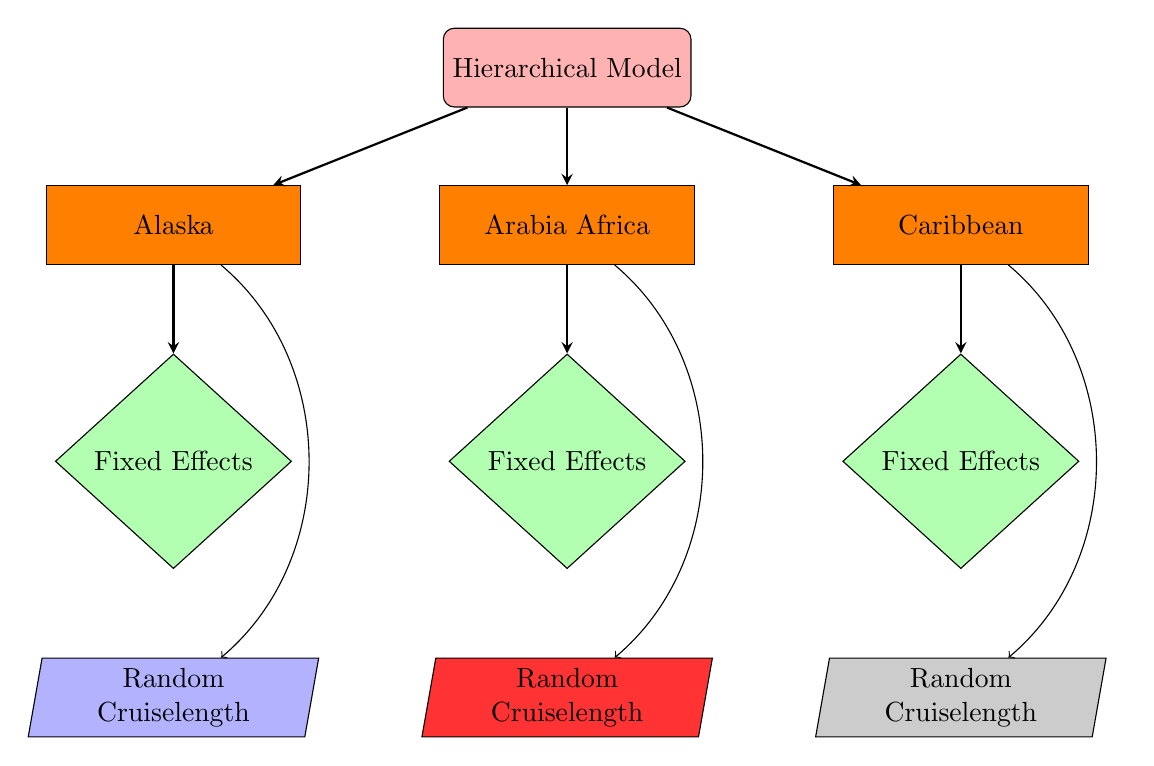
\begin{tikzpicture}[node distance=2cm][line/.style={<->,shorten >=0.4cm,shorten <=0.4cm},thick]

\node (model) [startstop] {Hierarchical Model};

\node (arabia) [process, below of=model] {Arabia Africa};
\node (alaska) [process, left of=arabia, node distance = 5cm] {Alaska};
\node (caribbean) [process, right of=arabia, node distance = 5cm] {Caribbean};
\node (fixedAlaska) [fixedEffects, below of=alaska] {Fixed Effects};
\node (fixedArabia) [fixedEffects, below of=arabia] {Fixed Effects};
\node (fixedCaribbean) [fixedEffects, below of=caribbean] {Fixed Effects};
\node (randomAlas) [randomAlaska, below of=fixedAlaska] {Random Cruiselength};
\node (randomArab) [randomArabia, below of=fixedArabia] {Random Cruiselength};
\node (randomCar) [randomCaribbean, below of=fixedCaribbean] {Random Cruiselength};

\draw [arrow] (model) -- (arabia);
\draw [arrow] (model) -- (alaska);
\draw [arrow] (model) -- (caribbean);
\draw [arrow] (arabia) -- (fixedArabia);
\draw [arrow] (alaska) -- (fixedAlaska);
\draw [arrow] (caribbean) -- (fixedCaribbean);
\path [->] (alaska) edge [bend left=50]  (randomAlas);
\path [->] (arabia) edge [bend left=50]  (randomArab);
\path [->] (caribbean) edge [bend left=50]  (randomCar);
\end{tikzpicture}\\

\begin{table}[H]
	\centering
	\caption{Random Effects For Each Trade}
\begin{tabular}{rrrr}

	       &(Intercept) & PAX AGE & CRUISELENGTH \\
	       \hline
	       \hline
	ALASKA & 27.200 & -0.195 & -0.372 \\
	ARABIA  AFRICA & 1.868 & -0.0565 & 0.0616 \\
	ASIA  ORIENT & 5.466 & 0.099 & -0.186 \\
	BERMUDA & -6.890 & -0.062 & 0.195 \\
	CANADA NEW ENGLAND & 2.968 & 0.025 & -0.146 \\
	CARIBBEAN & 0.602 & -0.135 & 0.281 \\
	COASTAL & -7.058 & -0.055 & 0.122 \\
	EUROPE & 4.038 & 0.098 & -0.219 \\
	HAWAII & 0.601 & -0.091 & 0.069 \\
	MEXICO & -3.723 & -0.135 & 0.240 \\
	PANAMA  CANAL & 8.025 & -0.113 & -0.061 \\
	SOUTH  AMERICA & 24.446 & -0.097 & -0.331 \\
	SOUTH  PACIFIC & 1.423 & 0.075 & -0.335 \\
	WORLD  VOYAGE & 3.117 & -0.042 & 0.048 \\
	\hline 
	\hline 
\end{tabular}
\end{table}


\begin{table}[H]
	\centering
		\scalebox{.8}{
\begin{tabular}{rrrrrr}
	TRADE & MSE  H-Model & MSE  L-Model & Root  MSE  H-Model & Root  MSE  L-Model & Difference  (H  -  L) \\
	\hline
	\hline 
	ALASKA & 142916033.05 & 142950093.176 & 11954.749 & 11956.174 & -1.424 \\
	ARABIA  AFRICA & 139177.901 & 138428.29 & 373.066 & 372.06 & 1.006 \\
	ASIA  ORIENT & 12599774.516 & 12607344.433 & 3549.616 & 3550.682 & -1.066 \\
	BERMUDA & 990319.344 & 991735.717 & 995.148 & 995.859 & -0.711 \\
	CANADA  NEW  ENGLAND & 12375936.024 & 12383713.406 & 3517.945 & 3519.05 & -1.105 \\
	CARIBBEAN & 26034314.381 & 26127430.983 & 5102.383 & 5111.5 & -9.117 \\
	COASTAL & 232540.77 & 237522.834 & 482.225 & 487.363 & -5.138 \\
	EUROPE & 112695242.718 & 112879226.001 & 10615.802 & 10624.464 & -8.662 \\
	HAWAII & 1213897.316 & 1215500.332 & 1101.77 & 1102.497 & -0.727 \\
	MEXICO & 1049953.72 & 1050385.965 & 1024.672 & 1024.883 & -0.211 \\
	PANAMA  CANAL & 1912796.293 & 1918003.148 & 1383.039 & 1384.92 & -1.881 \\
	SOUTH  AMERICA & 11101312.152 & 11155591.93 & 3331.863 & 3339.999 & -8.136 \\
	SOUTH  PACIFIC & 11816475.402 & 11922887.925 & 3437.51 & 3452.954 & -15.443 \\
	WORLD  VOYAGE & 1302341.706 & 1402538.175 & 1141.202 & 1184.288 & -43.086 \\
	\hline 
	\hline 
\end{tabular}
}
\caption{Shorex estimations}
\end{table}

\begin{table}[H]
	\centering
	\scalebox{.8}{
\begin{tabular}{rrrrrr}
	TRADE & MSE  H-Model & MSE  L-Model & Root  MSE  H-Model & Root  MSE L-Model & Difference (H - L) \\
	\hline 
	\hline 
	ALASKA & 24022216.982 & 24020666.807 & 4901.246 & 4901.088 & 0.158 \\
	ARABIA  AFRICA & 17063.335 & 17181.196 & 130.627 & 131.077 & -0.45 \\
	ASIA ORIENT & 1732959.016 & 1742196.889 & 1316.419 & 1319.923 & -3.504 \\
	BERMUDA & 609719.437 & 609812.224 & 780.845 & 780.905 & -0.059 \\
	CANADA NEW ENGLAND & 3949370.849 & 3950653.567 & 1987.302 & 1987.625 & -0.323 \\
	CARIBBEAN & 22759856.624 & 22765269.872 & 4770.729 & 4771.296 & -0.567 \\
	COASTAL & 525528.197 & 582931.343 & 724.933 & 763.499 & -38.566 \\
	EUROPE & 16771197.483 & 16779542.059 & 4095.265 & 4096.284 & -1.019 \\
	HAWAII & 605653.636 & 611392.545 & 778.238 & 781.916 & -3.678 \\
	MEXICO & 973958.109 & 974590.248 & 986.893 & 987.213 & -0.32 \\
	PANAMA CANAL & 1281334.384 & 1283807.997 & 1131.96 & 1133.053 & -1.092 \\
	SOUTH AMERICA & 1230938.015 & 1231187.435 & 1109.476 & 1109.589 & -0.112 \\
	SOUTH PACIFIC & 2877253.544 & 2879071.23 & 1696.247 & 1696.783 & -0.536 \\
	WORLD VOYAGE & 132608.056 & 144673.15 & 364.154 & 380.359 & -16.205 \\
	\hline 
	\hline 
\end{tabular}
	}
	\caption{Bar estimations}
	\end{table}
	
\begin{table}[H]
	\scalebox{.8}{
	\begin{tabular}{rrrrrr}
		TRADE & MSE H-Model & MSE L-Model & Root MSE H-Model & Root MSE L-Model & Difference (H - L) \\
		\hline 
		\hline 
		ALASKA & 24022216.982 & 24020666.807 & 4901.246 & 4901.088 & 0.158 \\
		ARABIA AFRICA & 17063.335 & 17181.196 & 130.627 & 131.077 & -0.45 \\
		ASIA ORIENT & 1732959.016 & 1742196.889 & 1316.419 & 1319.923 & -3.504 \\
		BERMUDA & 609719.437 & 609812.224 & 780.845 & 780.905 & -0.059 \\
		CANADA NEW ENGLAND & 3949370.849 & 3950653.567 & 1987.302 & 1987.625 & -0.323 \\
		CARIBBEAN & 22759856.624 & 22765269.872 & 4770.729 & 4771.296 & -0.567 \\
		COASTAL & 525528.197 & 582931.343 & 724.933 & 763.499 & -38.566 \\
		EUROPE & 16771197.483 & 16779542.059 & 4095.265 & 4096.284 & -1.019 \\
		HAWAII & 605653.636 & 611392.545 & 778.238 & 781.916 & -3.678 \\
		MEXICO & 973958.109 & 974590.248 & 986.893 & 987.213 & -0.32 \\
		PANAMA CANAL & 1281334.384 & 1283807.997 & 1131.96 & 1133.053 & -1.092 \\
		SOUTH AMERICA & 1230938.015 & 1231187.435 & 1109.476 & 1109.589 & -0.112 \\
		SOUTH PACIFIC & 2877253.544 & 2879071.23 & 1696.247 & 1696.783 & -0.536 \\
		WORLD VOYAGE & 132608.056 & 144673.15 & 364.154 & 380.359 & -16.205 \\
		\hline 
		\hline 
	\end{tabular}
}
\caption{Photo estimations}
\end{table} 

\end{document}